\documentclass[11pt]{article}
% Shared preamble for the notes in this repository. pdfLaTeX, TeX Live 2024 or later.
\usepackage[a4paper,margin=2.6cm]{geometry}
\usepackage[T1]{fontenc}
\usepackage{lmodern}
\usepackage{microtype}
\usepackage{amsmath,amssymb,amsthm}
\usepackage{graphicx}
\usepackage{booktabs}
\usepackage{enumitem}
\usepackage[dvipsnames]{xcolor}
\usepackage[hidelinks]{hyperref}
\hypersetup{colorlinks=true,linkcolor=MidnightBlue,citecolor=MidnightBlue,urlcolor=MidnightBlue}
\graphicspath{{../../figures/}}
\setlist{itemsep=2pt,topsep=4pt}

\newtheorem{theorem}{Theorem}
\newtheorem{proposition}[theorem]{Proposition}
\newtheorem{corollary}[theorem]{Corollary}
\newtheorem{conjecture}[theorem]{Conjecture}
\theoremstyle{definition}
\newtheorem{definition}[theorem]{Definition}
% Reusable derivations, numbered note.k; each note sets \notenumber. Indexed in DERIVATIONS.md.
\newcommand{\notenumber}{0}
\newtheorem{derivation}{Derivation}
\renewcommand{\thederivation}{\notenumber.\arabic{derivation}}
\newtheorem{question}{Question}
\theoremstyle{remark}
\newtheorem{remark}[theorem]{Remark}

\newcommand{\Z}{\mathbb{Z}}
\newcommand{\Q}{\mathbb{Q}}
\newcommand{\R}{\mathbb{R}}
\newcommand{\C}{\mathbb{C}}
\newcommand{\HH}{\mathbb{H}}
\newcommand{\SL}{\mathrm{SL}}
\newcommand{\Gal}{\mathrm{Gal}}
\newcommand{\Hom}{\mathrm{Hom}}
\newcommand{\repo}{\href{https://github.com/rmorleysmith/l-functions-and-physics}{\texttt{l-functions-and-physics}}}
\newcommand{\formal}{\href{https://github.com/rmorleysmith/morley-smith-formal}{\texttt{morley-smith-formal}}}
\newcommand{\script}[1]{\href{https://github.com/rmorleysmith/l-functions-and-physics/blob/main/scripts/#1}{\texttt{scripts/#1}}}
% A path inside the Lean repository; it may break after a slash.
\newcommand{\leanpath}[1]{\nolinkurl{#1}}

% Grades used in every status table.
\newcommand{\gradeLean}{\textsc{lean}}      % proved in Lean 4 with Mathlib
\newcommand{\gradeClassical}{\textsc{classical}}  % a published theorem, cited
\newcommand{\gradeComputed}{\textsc{computed}}    % checked numerically by a script in this repository
\newcommand{\gradeConvention}{\textsc{convention}}  % a choice of units or names
\newcommand{\gradeOpen}{\textsc{open}}      % a question, conjecture or working hypothesis
% The legend printed under every status table.
\newcommand{\gradelegend}{\par\nopagebreak\smallskip\noindent\begin{minipage}{\textwidth}\small
\gradeLean: proved in Lean 4 with Mathlib.
\gradeClassical: a published theorem.
\gradeComputed: checked numerically by a script in the repository \repo.
\gradeConvention: a choice of units or names.
\gradeOpen: a question, conjecture or working hypothesis.
\end{minipage}\par\medskip}
% A plain-language physical reading, placed after each derivation.
\newcommand{\physical}{\paragraph{In physical terms.}}

\renewcommand{\notenumber}{6}

\title{Towards a number-theoretic standard model}
\author{Richard Morley-Smith}
\date{Note 06 \quad November 2026}

\begin{document}
\maketitle

\begin{abstract}
\noindent
We record four exact facts about the representations of the Standard Model of particle physics, each checked in rational arithmetic or in Lean, and then state the programme they suggest as a working hypothesis and five questions.
For one generation of fermions with quantised hypercharge, the conditions for the cancellation of gauge anomalies are Fermat's equation $x^3+y^3=z^3$, and its trivial solutions are the observed hypercharges (Lohitsiri and Tong); the same reduction holds for any number of colours.
The root lattice of the colour group is the ring of Eisenstein integers $\Z[\omega]$: its roots are the units, and its centre is the residue field $\Z[\omega]/(1-\omega)$.
The fields of the model are blind to a subgroup $\Z/6$ of the gauge group, and the abelianisation of $\mathrm{PSL}(2,\Z)$ is $\Z/6$.
The model is chiral; a Dirichlet character has a parity, and the cohomology of a modular form has two conjugate Hodge types.
The questions ask whether these are traces of one arithmetic structure, and what would have to be constructed for the answer to be yes.
\end{abstract}

\section{Balance: anomaly cancellation is Diophantine}\label{sec:balance}

Write one generation as left-handed Weyl fermions:

\begin{center}
\begin{tabular}{@{}lccrr@{}}
\toprule
field & $SU(3)$ & $SU(2)$ & $Y$ & $6Y$\\
\midrule
$Q$ & $\mathbf 3$ & $\mathbf 2$ & $\tfrac16$ & $1$\\
$u^c$ & $\bar{\mathbf 3}$ & $\mathbf 1$ & $-\tfrac23$ & $-4$\\
$d^c$ & $\bar{\mathbf 3}$ & $\mathbf 1$ & $\tfrac13$ & $2$\\
$L$ & $\mathbf 1$ & $\mathbf 2$ & $-\tfrac12$ & $-3$\\
$e^c$ & $\mathbf 1$ & $\mathbf 1$ & $1$ & $6$\\
\bottomrule
\end{tabular}
\end{center}

\noindent
A gauge theory with chiral fermions is consistent only if its gauge anomalies cancel \cite{Weinberg}.
For the Standard Model there are six conditions: $SU(3)^3$, $SU(3)^2U(1)$, $SU(2)^2U(1)$, $U(1)^3$, the mixed gravitational $U(1)$ condition, and Witten's $SU(2)$ condition (an even number of doublets) \cite{Witten}.
The script \script{standard\_model.py} checks all six in exact rational arithmetic.
The electric charges of a generation also sum to zero.

\paragraph{The conditions determine the hypercharges of a generation.}
Keep the representations of the fifteen fermions and let the hypercharges $y_Q,y_u,y_d,y_L,y_e$ be unknown.
The conditions read
\[
  2y_Q+y_u+y_d = 0,\quad 3y_Q+y_L=0,\quad 6y_Q+3y_u+3y_d+2y_L+y_e = 0,\quad 6y_Q^3+3y_u^3+3y_d^3+2y_L^3+y_e^3 = 0.
\]
The linear ones give $y_L=-3y_Q$, $y_e = 6y_Q$ and $y_u+y_d=-2y_Q$.
Then the cubic gives $y_Q\,(y_uy_d + 8y_Q^2) = 0$.
For $y_Q\ne0$ this is $\{y_u,y_d\} = \{2y_Q,-4y_Q\}$: the solution is unique up to scale and the exchange $u\leftrightarrow d$, and it is the observed one (Geng and Marshak \cite{GengMarshak}, Minahan, Ramond and Warner \cite{MRW}; see the account in \cite{LohitsiriTong}).
For $y_Q=0$ the solutions are $y_L=y_e=0$, $y_d=-y_u$, in which only the two quark singlets are charged, with opposite charges.
An exhaustive search over integers $|y|\le40$ with $y_Q = 1$ finds exactly the two observed solutions.

The statement concerns one generation of fifteen.
With a right-handed neutrino the four conditions hold for $Y+\varepsilon(B-L)$ for every $\varepsilon$, so the hypercharges of sixteen fermions are not fixed by them.
For three generations it holds when the generations carry equal charges; without that assumption the conditions are four equations in fifteen unknowns.
For a single $U(1)$ with $n$ charged Weyl fermions the corresponding equations, $\sum z_i = \sum z_i^3 = 0$ in integers, were solved in general by Costa, Dobrescu and Fox \cite{CDF} and, by a geometric method resting on elementary constructions of number theory, by Allanach, Gripaios and Tooby-Smith \cite{AGT}, who also treat an additional $U(1)$ in extensions of the Standard Model \cite{AGT2}.

\paragraph{Without gravity: Fermat's cubic.}
Drop the gravitational condition, the third of the four, and suppose that hypercharge is quantised: the gauge group is $U(1)$ and not $\R$, so that the hypercharges are rational multiples of one unit.
The two linear gauge conditions give $y_L = -3y_Q$ and $y_d = -2y_Q-y_u$, and the cubic condition becomes
\[
  y_e^3+(y_u-2y_Q)^3 = (y_u+4y_Q)^3,
\]
Fermat's equation of degree 3.
This is the theorem of Lohitsiri and Tong \cite{LohitsiriTong}; they reach Fermat's curve by a rational change of variables, and the polynomial form above is the one used in the Lean proof.
Its rational solutions are the trivial ones, in which one of the three cubes is zero (Euler; the proof in Mathlib is a descent in $\Z[\omega]$).
The three cases are the solution with $y_Q=0$ and the two assignments $\{y_u,y_d\} = \{2y_Q,-4y_Q\}$ with $y_e = 6y_Q$ found above.
In each case the gravitational condition holds.
So for quantised hypercharge the gauge conditions alone give the hypercharges, and the gravitational condition follows from them.
Quantisation is a hypothesis here: over the reals $(y_Q,y_u,y_d,y_L,y_e) = (1,0,-2,-3,\sqrt[3]{72})$ satisfies the gauge conditions and not the gravitational one.

That every rational solution of the gauge conditions satisfies the gravitational condition is proved in Lean in Physlib, by Tooby-Smith \cite{Physlib,HepLean}, from Mathlib's proof of Fermat's theorem for cubes.
The explicit list of solutions is proved in Lean in \formal{} (\leanpath{MorleySmithFormal/Hypercharge}), from the same theorem.

\paragraph{Any number of colours.}
With $N$ colours in place of three the gauge conditions are $2y_Q+y_u+y_d=0$, $Ny_Q+y_L=0$ and $2Ny_Q^3+Ny_u^3+Ny_d^3+2y_L^3+y_e^3=0$, and the same substitution gives
\[
  y_e^3+\bigl(y_u+(1-N)y_Q\bigr)^3 = \bigl(y_u+(N+1)y_Q\bigr)^3 .
\]
The reduction to Fermat's cubic holds for every $N$: the exponent is that of the triangle diagram, and the number of colours enters through the coefficients.
The solutions with $y_Q\neq0$ are $\{y_u,y_d\} = \{(N-1)y_Q,\,-(N+1)y_Q\}$, $y_L=-Ny_Q$, $y_e=2Ny_Q$, and they satisfy the gravitational condition.
The list of solutions and the gravitational consequence for every $N\ge1$ are proved in Lean in the same file.

\physical
Once the fermions of a generation are fixed and hypercharge is quantised, consistency fixes the hypercharges up to one scale.
The electric charges follow when the Higgs doublet is added: with $y_u=-4y_Q$ the Yukawa coupling of $Q$ and $u^c$ fixes its hypercharge, $y_H = -y_Q-y_u = 3y_Q$, the charge left unbroken is $T_3+Y/(2y_H)$, and it takes the values $\frac23$ and $-\frac13$ on the quarks and $0$ and $-1$ on the leptons.

\section{Colour lives on the Eisenstein integers}\label{sec:colour}

In the plane, the roots of $SU(3)$ are the six units $\pm1,\pm\omega,\pm\omega^2$ of $\Z[\omega]$, with Cartan matrix $\left(\begin{smallmatrix}2&-1\\-1&2\end{smallmatrix}\right)$.
So the colour root lattice is the ring of Eisenstein integers, the hexagonal lattice of notes~01 and~02 \cite{ConwaySloane}.
The six roots are six of the eight gluons, and the other two have weight zero.
The highest weight of the quark triplet is $1/(1-\omega)$.
The three colours are $1/(1-\omega)$ times the cube roots of unity $1,\omega,\omega^2$, and the antiquarks are their negatives (Figure~\ref{fig:colour}, left).
The weight lattice is $(1-\omega)^{-1}\Z[\omega]$, and its index over the root lattice is $N(1-\omega) = 3$, the determinant of the Cartan matrix.
So the centre $\Z/3$ of $SU(3)$ is the residue field $\Z[\omega]/(1-\omega)$ at the ramified prime $\sqrt{-3}$.

The six units are also the stabiliser of the Eisenstein point of note~01.
The element $ST$ fixes $\rho$ and acts on the lattice $\Z+\Z\rho$ as multiplication by $\rho+1 = e^{2\pi i/6}$, so the six roots are one orbit of the stabiliser of $\rho$.
In the same way the roots of the weak $SU(2)$ are the units $\pm1$ of $\Z$.
The eight gauge bosons of non-zero weight, six gluons and $W^\pm$, are indexed by the units of $\Z[\omega]$ and of $\Z$, and the four of weight zero by the rank $2+1+1$.
The script checks each of these statements.

The same ring carries the descent that proves Fermat's theorem for cubes.
For $N$ colours the cubic of Section~\ref{sec:balance} is unchanged while the root lattice becomes $A_{N-1}$, so the two appearances of $\Z[\omega]$ meet at $N=3$ only.

\begin{question}\label{q:colour}
Is there a construction in which the root lattice of colour and the lattice $\Z+\Z\rho$ on which the stabiliser of $\rho$ acts are one lattice, with the six roots and the six units matched by the construction and not only by their coordinates?
\end{question}

\begin{figure}[ht]
  \centering
  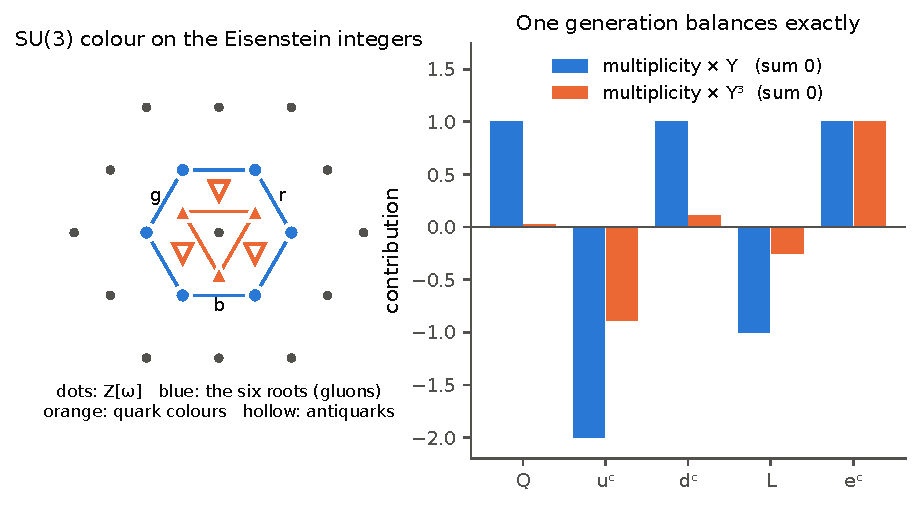
\includegraphics[width=0.95\textwidth]{sm-colour-balance}
  \caption{Left: the six roots of $SU(3)$ are the units of $\Z[\omega]$; quark colours are $1/(1-\omega)$ times the cube roots of unity. Right: each field's contribution to the linear and cubic anomaly conditions; each set sums to zero.}
  \label{fig:colour}
\end{figure}

\section{The hidden $\Z/6$}

The element $(e^{2\pi i/3}I_3,\,-I_2,\,e^{2\pi i/6})$ of $SU(3)\times SU(2)\times U(1)$ acts trivially on every field of the Standard Model, the Higgs included.
The subgroup that acts trivially is exactly the $\Z/6$ it generates.
So the group acting faithfully on the fields is $(SU(3)\times SU(2)\times U(1))/\Z_6$ \cite{BaezHuerta}.
Which quotient by a subgroup of $\Z/6$ is nature's gauge group is an open question in physics \cite{Tong}.
This $\Z/6$ projects onto the centre $\Z/2$ of $SU(2)$ and onto the centre $\Z/3$ of $SU(3)$.
On the arithmetic side, $\mathrm{PSL}(2,\Z) = \Z/2*\Z/3$ has abelianisation $\Z/6 = \Z/2\times\Z/3$, the two factors generated by the images of $S$ and $ST$.
Equivalently, the characters of $\SL(2,\Z)$ trivial on $-1$ are the six even powers of the $\eta^2$ multiplier (note~01).

\begin{question}\label{q:six}
The two groups of order six are isomorphic, in two ways.
Is one of the two isomorphisms induced by a homomorphism from $\mathrm{PSL}(2,\Z)$ to the gauge group that arises from the construction asked for in Question~\ref{q:colour}?
\end{question}

\section{Particles as representations}

By Wigner's classification a particle is an irreducible unitary representation of the Poincar\'e group, and its mass squared is the eigenvalue of a Casimir operator \cite{Wigner}.
Automorphic forms offer an analogy.
An automorphic form generates an irreducible representation of $\SL(2,\R)$, or of an adelic group \cite{Bump}.
For a Maass form the Casimir eigenvalue is the Laplace eigenvalue $\frac14+r^2$, and it stands in the place of a mass.
For a holomorphic form of weight $k$, the weight, the character by which the rotation subgroup $SO(2)$ acts, stands in the place of spin.
Hecke eigenvalues stand in the place of charges, and the $L$-function packages them.

\begin{question}\label{q:rep}
Is there an $L$-function, built from automorphic representations attached to the particles of the Standard Model, from which a number of the model can be derived, such as the number of generations or a ratio of masses?
\end{question}

\section{Handedness}

Each side has a two-fold structure, and the three are of different kinds.
\begin{enumerate}
\item \emph{Characters.} A Dirichlet character $\chi$ is even or odd, according to $\chi(-1)=\pm1$.
The characters of imaginary quadratic fields are odd, and the parity sets the gamma factor of the $L$-function (note~04).
This is a grading by $\Z/2$.
\item \emph{Modular forms.} For $\SL(2,\Z)$ and weight $k$ the parabolic cohomology is isomorphic to $S_k\times S_k$, through the even and odd period polynomials (Eichler and Shimura).
The classes of the period polynomials of cusp forms span a subspace $H^{k-1,0}$ that is complementary to its complex conjugate $H^{0,k-1}$.
Both statements are proved in Lean, in files that accompany the results of \formal{} (\leanpath{tau-track/TauTrack/Cohomology}).
Conjugation exchanges the two parts, so the pair is symmetric under conjugation.
\item \emph{The Standard Model.} $SU(2)$ acts only on left-handed fermions, and the representation of a generation is not equivalent to its conjugate.
The script checks this.
This is chirality in the sense of physics.
\end{enumerate}

\begin{question}\label{q:chiral}
Chirality in the third item says that a representation differs from its conjugate.
Is there an object on the arithmetic side whose representation differs from its conjugate in this sense, and to which the parity of the first item and the two Hodge types of the second are related?
\end{question}

\section{The programme}

The facts above are the fixed points of a programme, which we state as a working hypothesis: \emph{the Standard Model is arithmetic}.
In detail: its particles are stable signatures of a lattice-like arithmetic space; its gauge group $SU(3)\times SU(2)\times U(1)$, whose three factors are mutually orthogonal and whose charges balance, reflects the structure of the modular group; the whole is described by an $L$-function; and handedness enters at every level, from the characters upward.
The terms have exact meanings.
\begin{itemize}
\item \emph{Torsion.} A torsion element of a group is one of finite order.
$\SL(2,\Z)$ is generated by the torsion elements $S$ and $ST$, and its twelve characters are determined by their values on these two (note~01).
The coupling between lattices that the programme also calls torsion is to be made precise.
\item \emph{Bosons.} The model has twelve gauge bosons of spin~1 (eight gluons, $W^\pm$, $Z$ and the photon) and one scalar, the Higgs boson, whose field gives mass to the fermions and to $W^\pm$ and $Z$.
\item \emph{Orthogonal.} The Lie algebra $\mathfrak{su}(3)\oplus\mathfrak{su}(2)\oplus\mathfrak{u}(1)$ is an orthogonal direct sum for its invariant inner product.
\item \emph{Balance.} The charges satisfy the anomaly-cancellation equations of Section~\ref{sec:balance}.
\item \emph{A stable signature.} A particle is an irreducible representation, and its mass is a Casimir eigenvalue (Wigner).
\end{itemize}
Questions~\ref{q:colour} to~\ref{q:chiral} ask for the constructions that would turn the hypothesis into statements.
One further coincidence of counts started the programme.
There are twelve fermion flavours, four in each of three generations: six quarks ($u,d,c,s,t,b$) and six leptons ($e,\mu,\tau$ and three neutrinos).
There are twelve gauge bosons, since $\dim SU(3)+\dim SU(2)+\dim U(1) = 8+3+1$.
The modular group has twelve characters (note~01).

\begin{question}\label{q:twelve}
Do the three twelves have a common origin?
A positive answer would derive the number of generations and the dimension $8+3+1$ from the modular group.
\end{question}

\section*{Status of the statements}

\begin{center}
\small
\begin{tabular}{@{}p{0.66\textwidth}l@{}}
\toprule
Statement & Grade\\
\midrule
The six anomaly conditions hold for one generation & \gradeClassical, \gradeComputed\\
With gravity they fix the hypercharges of a generation of fifteen, for $y_Q\ne0$, up to scale and $u\leftrightarrow d$ & \gradeClassical, \gradeComputed\\
For rational hypercharges the gauge conditions alone are Fermat's cubic; their solutions; they imply the gravitational condition (the last also in Physlib) & \gradeClassical, \gradeLean\\
The same for $N$ colours: the cubic, the solutions, the gravitational condition & \gradeLean, \gradeComputed\\
The real solution without the gravitational condition; the family $Y+\varepsilon(B-L)$; the electric charges with the Higgs & \gradeComputed\\
$SU(3)$ roots are the units of $\Z[\omega]$; centre $=\Z[\omega]/(1-\omega)$ & \gradeClassical, \gradeComputed\\
The roots are one orbit of the stabiliser of $\rho$ & \gradeComputed\\
The fields are blind to $\Z/6$ & \gradeClassical, \gradeComputed\\
$\mathrm{PSL}(2,\Z)^{\mathrm{ab}} = \Z/6$ (a consequence of the Lean statement of note~01) & \gradeComputed\\
Parabolic cohomology of $\SL(2,\Z)$ is $S_k\times S_k$; the Hodge decomposition (accompanying files, without a Challenge statement) & \gradeClassical, \gradeLean\\
A generation is not equivalent to its conjugate & \gradeComputed\\
The working hypothesis and Questions~\ref{q:colour}--\ref{q:twelve} & \gradeOpen\\
\bottomrule
\end{tabular}
\end{center}
\gradelegend

\begin{thebibliography}{99}
\bibitem{AGT} B.~C. Allanach, B.~Gripaios and J.~Tooby-Smith, Geometric general solution to the $U(1)$ anomaly equations, \emph{J. High Energy Phys.} 2020, no.~5, 065.
\bibitem{AGT2} B.~C. Allanach, B.~Gripaios and J.~Tooby-Smith, Solving local anomaly equations in gauge-rank extensions of the Standard Model, \emph{Phys. Rev. D} 101 (2020), 075015.
\bibitem{BaezHuerta} J.~Baez and J.~Huerta, The algebra of grand unified theories, \emph{Bull. Amer. Math. Soc.} 47 (2010), 483--552.
\bibitem{Bump} D.~Bump, \emph{Automorphic Forms and Representations}, Cambridge University Press, 1997.
\bibitem{ConwaySloane} J.~H. Conway and N.~J.~A. Sloane, \emph{Sphere Packings, Lattices and Groups}, 3rd ed., Springer, 1999.
\bibitem{CDF} D.~B. Costa, B.~A. Dobrescu and P.~J. Fox, General solution to the $U(1)$ anomaly equations, \emph{Phys. Rev. Lett.} 123 (2019), 151601.
\bibitem{GengMarshak} C.~Q. Geng and R.~E. Marshak, Uniqueness of quark and lepton representations in the standard model from the anomalies viewpoint, \emph{Phys. Rev. D} 39 (1989), 693--696.
\bibitem{LohitsiriTong} N.~Lohitsiri and D.~Tong, Hypercharge quantisation and Fermat's last theorem, \emph{SciPost Phys.} 8 (2020), 009.
\bibitem{MRW} J.~A. Minahan, P.~Ramond and R.~C. Warner, Comment on anomaly cancellation in the standard model, \emph{Phys. Rev. D} 41 (1990), 715--716.
\bibitem{Physlib} J.~Tooby-Smith, theorem \texttt{SM.SMNoGrav.One.accGravSatisfied}, in The Physlib Community, \emph{Physlib: the Lean physics library}, \url{https://github.com/leanprover-community/physlib}, file \nolinkurl{Physlib/Particles/StandardModel/AnomalyCancellation/NoGrav/One/Lemmas.lean}.
\bibitem{HepLean} J.~Tooby-Smith, HepLean: digitalising high energy physics, \emph{Comput. Phys. Commun.} 308 (2025), 109457.
\bibitem{Tong} D.~Tong, Line operators in the Standard Model, \emph{J. High Energy Phys.} 2017, no.~7, 104.
\bibitem{Weinberg} S.~Weinberg, \emph{The Quantum Theory of Fields}, vol.~2, Cambridge University Press, 1996.
\bibitem{Wigner} E.~P. Wigner, On unitary representations of the inhomogeneous Lorentz group, \emph{Ann. of Math.} 40 (1939), 149--204.
\bibitem{Witten} E.~Witten, An $SU(2)$ anomaly, \emph{Phys. Lett. B} 117 (1982), 324--328.
\end{thebibliography}

\end{document}
